\documentclass[10pt,a4paper]{elsarticle}
\usepackage[margin=0.5in]{geometry}
\usepackage{amssymb}
\usepackage{subfig}
\usepackage{float}
%\usepackage{subfigure}
\usepackage{hyperref}
\hypersetup{colorlinks=true,linkcolor=blue}
\usepackage{amsmath}
\usepackage{bm}
\usepackage{tikz}
\usepackage{lipsum}
\usetikzlibrary{arrows.meta}
\usetikzlibrary{arrows}
\usepackage{pstricks}
\usetikzlibrary{patterns}
\usetikzlibrary{fadings}
\usetikzlibrary{shapes.geometric}
%\usepackage{graphicx}
% \usepackage[nodots,nocompress]{numcompress}
 	\definecolor{ig}{rgb}{0.07, 0.53, 0.03}
 	\definecolor{cd}{rgb}{0.89, 0.0, 0.13}






\begin{document}
\begin{figure}[t] %Needs to be modified!!!!!!!!!!!!!!!!
\centering
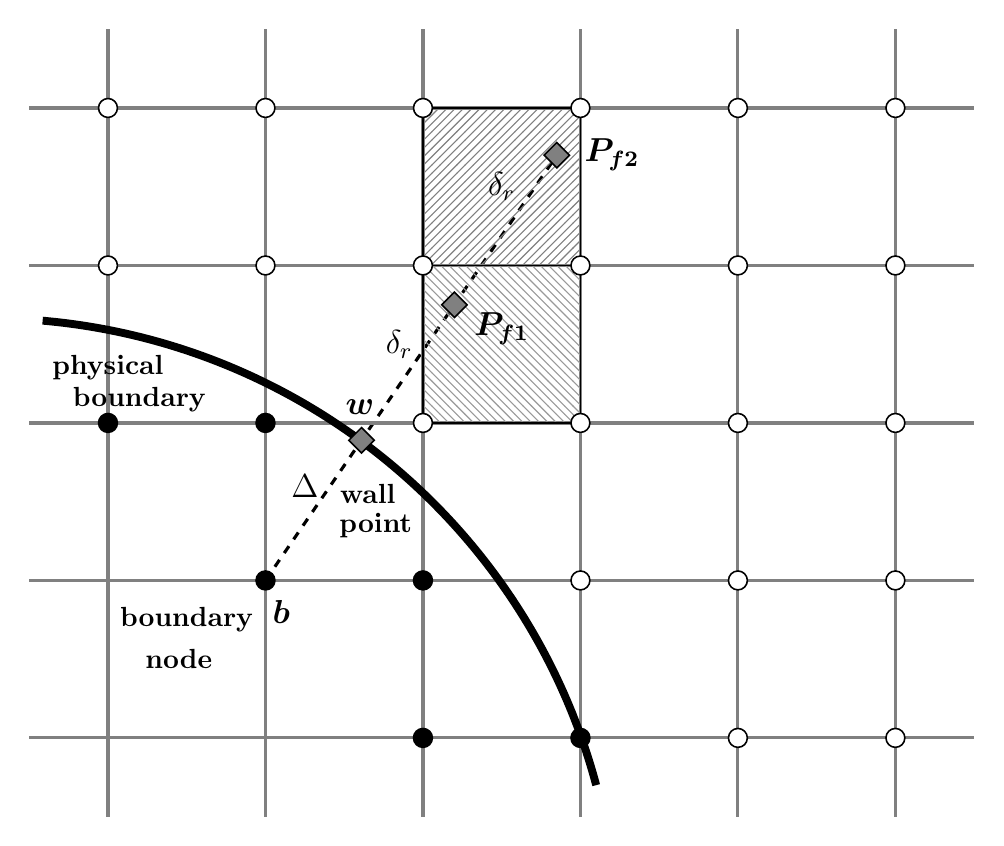
\begin{tikzpicture}[line width=0.2mm]
\draw[dashed,thick,line width=0.4mm] (4,2) -- (7.7,7.4);

\draw[gray,solid,thick,line width=0.4mm] (1,0) -- (13,0);
\draw[gray,solid,thick,line width=0.4mm] (1,2) -- (13,2);
\draw[gray,solid,thick,line width=0.4mm] (1,4) -- (13,4);
\draw[gray,solid,thick,line width=0.4mm] (1,6) -- (13,6);
\draw[gray,solid,thick,line width=0.4mm] (1,8) -- (13,8);

\draw[gray,solid,thick,line width=0.4mm] (2,-1) -- (2,9);
\draw[gray,solid,thick,line width=0.4mm] (4,-1) -- (4,9);
\draw[gray,solid,thick,line width=0.4mm] (6,-1) -- (6,9);
\draw[gray,solid,thick,line width=0.4mm] (8,-1) -- (8,9);
\draw[gray,solid,thick,line width=0.4mm] (10,-1) -- (10,9);
\draw[gray,solid,thick,line width=0.4mm] (12,-1) -- (12,9);

\draw[thick,line width=1mm] (8.2,-0.6) arc[start angle=15, end angle=85, radius=8];
\draw[pattern=north west lines, pattern color=gray!80] (6,4) rectangle (8,6);
\draw[pattern=north east lines, pattern color=gray] (6,6) rectangle (8,8);

%top first row
\draw[black,fill=white] (2,8)node[]{} circle(0.12cm);
\draw[black,fill=white] (4,8)node[]{} circle(0.12cm);
\draw[black,fill=white] (6,8)node[]{} circle(0.12cm);
\draw[black,fill=white] (8,8)node[]{} circle(0.12cm);
\draw[black,fill=white] (10,8)node[]{} circle(0.12cm);
\draw[black,fill=white] (12,8)node[]{} circle(0.12cm);

%top second row
\draw[black,fill=white] (2,6)node[]{} circle(0.12cm);
\draw[black,fill=white] (4,6)node[]{} circle(0.12cm);
\draw[black,fill=white] (6,6)node[]{} circle(0.12cm);
\draw[black,fill=white] (8,6)node[]{} circle(0.12cm);
\draw[black,fill=white] (10,6)node[]{} circle(0.12cm);
\draw[black,fill=white] (12,6)node[]{} circle(0.12cm);

%top third row
\draw[black,fill=black] (2,4)node[]{} circle(0.12cm);
\draw[black,fill=black] (4,4)node[]{} circle(0.12cm);
\draw[black,fill=white] (6,4)node[]{} circle(0.12cm);
\draw[black,fill=white] (8,4)node[]{} circle(0.12cm);
\draw[black,fill=white] (10,4)node[]{} circle(0.12cm);
\draw[black,fill=white] (12,4)node[]{} circle(0.12cm);

%top fourth row
\draw[black,fill=black] (4,2)node[]{} circle(0.12cm);
\draw[black,fill=black] (6,2)node[]{} circle(0.12cm);
\draw[black,fill=white] (8,2)node[]{} circle(0.12cm);
\draw[black,fill=white] (10,2)node[]{} circle(0.12cm);
\draw[black,fill=white] (12,2)node[]{} circle(0.12cm);

%top fifth row
\draw[black,fill=black] (6,0)node[]{} circle(0.12cm);
\draw[black,fill=black] (8,0)node[]{} circle(0.12cm);
\draw[black,fill=white] (10,0)node[]{} circle(0.12cm);
\draw[black,fill=white] (12,0)node[]{} circle(0.12cm);

\node [draw, fill=gray,diamond, aspect=1,scale=0.7] at (5.22,3.78) {};
\node [draw, fill=gray,diamond, aspect=1,scale=0.7] at (6.4,5.5) {};
\node [draw, fill=gray,diamond, aspect=1,scale=0.7] at (7.7,7.4) {};

\draw (7,5.2)node[]{\large{$\bm{P_{f1}}$}};
\draw (8.4,7.4)node[]{\large{$\bm{P_{f2}}$}};


\draw (5.7,5)node[]{\large{$\delta_r$}};
\draw (7,7)node[]{\large{$\delta_r$}};
\draw (4.5,3.2)node[]{\large{$\Delta$}};


\draw (4.2,1.6)node[]{\large{$\bm{b}$}};
\draw (3,1.5)node[]{\textbf{boundary}};
\draw (2.9,1)node[]{\textbf{node}};

% \draw (5.8,4.3)node[]{\large{$\bm{f}$}};
% \draw (6.8,3.6)node[]{\textbf{fluid}};
% \draw (6.8,3.1)node[]{\textbf{node}};


% \draw (7.6,6.3)node[]{\large{$\bm{ff}$}};

\draw (5.2,4.2)node[]{\large{$\bm{w}$}};
\draw (5.3,3.1)node[]{\textbf{wall}};
\draw (5.4,2.7)node[]{\textbf{point}};

\draw (2,4.7)node[]{\textbf{physical}};
\draw (2.4,4.3)node[]{\textbf{boundary}};

\end{tikzpicture}
\caption{Interpolation}
\end{figure}


\begin{figure}[t] %Needs to be modified!!!!!!!!!!!!!!!!
\centering
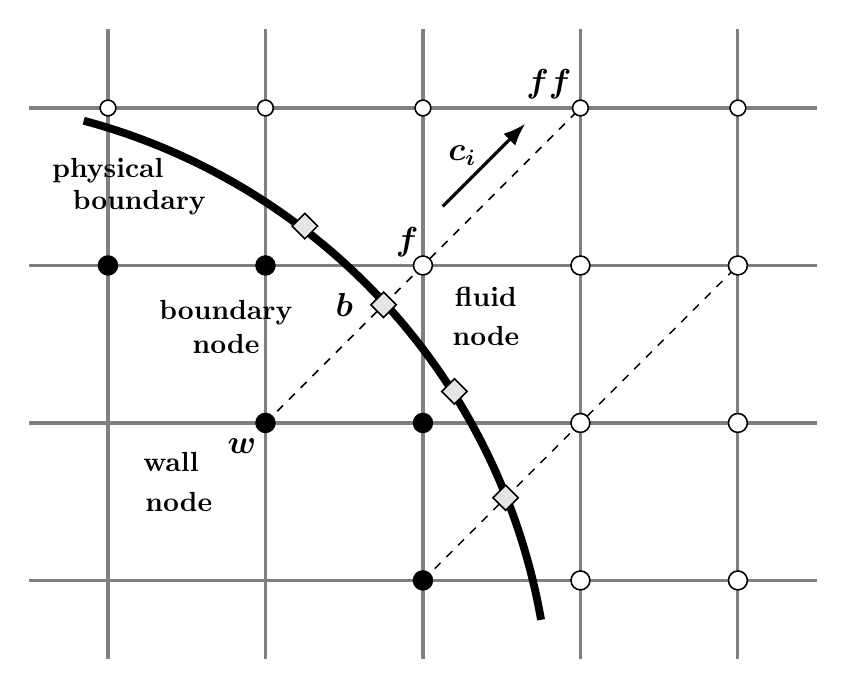
\begin{tikzpicture}[line width=0.2mm]
\draw[dashed] (4,2) -- (8,6);
\draw[dashed] (6,0) -- (10,4);

%\draw [dashed,line width=0.5mm] (0,0) rectangle(12,8);
\draw[gray,solid,thick,line width=0.4mm] (1,0) -- (11,0);
\draw[gray,solid,thick,line width=0.4mm] (1,2) -- (11,2);
\draw[gray,solid,thick,line width=0.4mm] (1,4) -- (11,4);
\draw[gray,solid,thick,line width=0.4mm] (1,6) -- (11,6);

\draw[gray,solid,thick,line width=0.4mm] (2,-1) -- (2,7);
\draw[gray,solid,thick,line width=0.4mm] (4,-1) -- (4,7);
\draw[gray,solid,thick,line width=0.4mm] (6,-1) -- (6,7);
\draw[gray,solid,thick,line width=0.4mm] (8,-1) -- (8,7);
\draw[gray,solid,thick,line width=0.4mm] (10,-1) -- (10,7);

\draw[thick,line width=1mm] (7.5,-0.5) arc[start angle=10, end angle=75, radius=8];

\draw[black,fill=white] (6,4)node[]{} circle(0.12cm);
% \draw[black,fill=white] (6,2)node[]{} circle(0.1cm);
\draw[black,fill=white] (8,2)node[]{} circle(0.12cm);
\draw[black,fill=white] (10,2)node[]{} circle(0.12cm);
\draw[black,fill=white] (8,4)node[]{} circle(0.12cm);
\draw[black,fill=white] (10,4)node[]{} circle(0.12cm);
\draw[black,fill=white] (8,0)node[]{} circle(0.12cm);
\draw[black,fill=white] (10,0)node[]{} circle(0.12cm);

\node [draw, fill=gray!20,diamond, aspect=1,scale=0.7] at (5.5,3.5) {};
\node [draw, fill=gray!20,diamond, aspect=1,scale=0.7] at (7.05,1.05) {};
\node [draw, fill=gray!20,diamond, aspect=1,scale=0.7] at (6.4,2.4) {};
\node [draw, fill=gray!20,diamond, aspect=1,scale=0.7] at (4.5,4.5) {};
% \node [draw, fill=white,diamond, aspect=1,scale=0.5] at (6,4) {};

\draw[black,fill=black] (6,0)node[]{} circle(0.12cm);
\draw[black,fill=black] (4,2)node[]{} circle(0.12cm);
\draw[black,fill=black] (2,4)node[]{} circle(0.12cm);
\draw[black,fill=black] (4,4)node[]{} circle(0.12cm);
\draw[black,fill=black] (6,2)node[]{} circle(0.12cm);



\draw[black,fill=white] (2,6)node[]{} circle(0.1cm);
\draw[black,fill=white] (4,6)node[]{} circle(0.1cm);
\draw[black,fill=white] (6,6)node[]{} circle(0.1cm);
\draw[black,fill=white] (8,6)node[]{} circle(0.1cm);
\draw[black,fill=white] (10,6)node[]{} circle(0.1cm);



\draw (3.7,1.7)node[]{\large{$\bm{w}$}};
\draw (2.8,1.5)node[]{\textbf{wall}};
\draw (2.9,1)node[]{\textbf{node}};

\draw (5.8,4.3)node[]{\large{$\bm{f}$}};
\draw (6.8,3.6)node[]{\textbf{fluid}};
\draw (6.8,3.1)node[]{\textbf{node}};


\draw (7.6,6.3)node[]{\large{$\bm{ff}$}};

\draw (5,3.5)node[]{\large{$\bm{b}$}};
\draw (3.5,3.4)node[]{\textbf{boundary}};
\draw (3.5,3)node[]{\textbf{node}};

\draw (2,5.2)node[]{\textbf{physical}};
\draw (2.4,4.8)node[]{\textbf{boundary}};

\draw[-Latex,shorten <=-2pt,solid,line width=0.4mm] (6.3,4.8) -- (7.3,5.8); %1
\draw (6.5,5.4)node[]{\large{$\bm{c_i}$}};

\end{tikzpicture}
\caption{Interpolation 2}
\end{figure}




\begin{figure}[t] %Needs to be modified!!!!!!!!!!!!!!!!
\centering
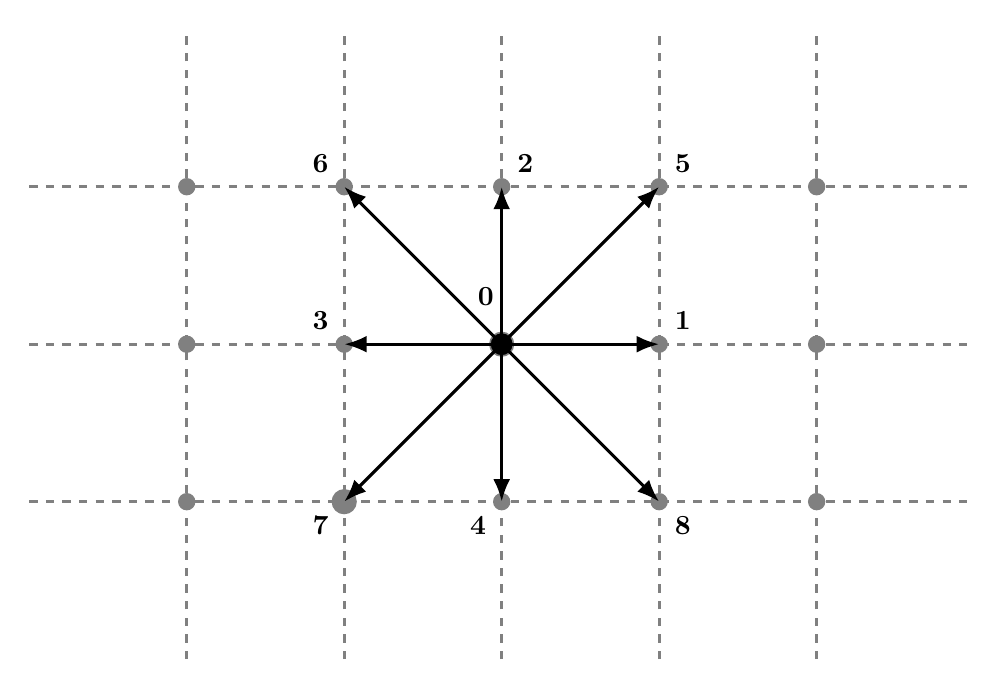
\begin{tikzpicture}[line width=0.2mm]
%\draw [dashed,line width=0.5mm] (0,0) rectangle(12,8);
\draw[gray,dashed,thick,line width=0.4mm] (0,2) -- (12,2);
\draw[gray,dashed,thick,line width=0.4mm] (0,4) -- (12,4);
\draw[gray,dashed,thick,line width=0.4mm] (0,6) -- (12,6);
\draw[gray,dashed,thick,line width=0.4mm] (2,0) -- (2,8);
\draw[gray,dashed,thick,line width=0.4mm] (4,0) -- (4,8);
\draw[gray,dashed,thick,line width=0.4mm] (6,0) -- (6,8);
\draw[gray,dashed,thick,line width=0.4mm] (8,0) -- (8,8);
\draw[gray,dashed,thick,line width=0.4mm] (10,0) -- (10,8);

\draw[gray,fill=black] (6,4)node[]{} circle(0.15cm);
\draw[gray,fill=gray] (2,2)node[]{} circle(0.1cm);
\draw[gray,fill=gray] (4,2)node[]{} circle(0.15cm);
\draw[gray,fill=gray] (6,2)node[]{} circle(0.1cm);
\draw[gray,fill=gray] (8,2)node[]{} circle(0.1cm);
\draw[gray,fill=gray] (10,2)node[]{} circle(0.1cm);

\draw[gray,fill=gray] (2,4)node[]{} circle(0.1cm);
\draw[gray,fill=gray] (4,4)node[]{} circle(0.1cm);
%\draw[black,fill=black] (6,4)node[]{} circle(0.15cm);
\draw[gray,fill=gray] (8,4)node[]{} circle(0.1cm);
\draw[gray,fill=gray] (10,4)node[]{} circle(0.1cm);

\draw[gray,fill=gray] (2,6)node[]{} circle(0.1cm);
\draw[gray,fill=gray] (4,6)node[]{} circle(0.1cm);
\draw[gray,fill=gray] (6,6)node[]{} circle(0.1cm);
\draw[gray,fill=gray] (8,6)node[]{} circle(0.1cm);
\draw[gray,fill=gray] (10,6)node[]{} circle(0.1cm);


\draw[-Latex,shorten <=-2pt,solid,line width=0.4mm] (6,4) -- (8,4); %1
\draw[-Latex,shorten <=-2pt,solid,line width=0.4mm] (6,4) -- (4,4); %3
\draw[-Latex,shorten <=-2pt,solid,line width=0.4mm] (6,4) -- (6,6); %2
\draw[-Latex,shorten <=-2pt,solid,line width=0.4mm] (6,4) -- (6,2); %4
\draw[-Latex,shorten <=-2pt,solid,line width=0.4mm] (6,4) -- (8,6); %5
\draw[-Latex,shorten <=-2pt,solid,line width=0.4mm] (6,4) -- (4,6); %5
\draw[-Latex,shorten <=-2pt,solid,line width=0.4mm] (6,4) -- (4,2); %7
\draw[-Latex,shorten <=-2pt,solid,line width=0.4mm] (6,4) -- (8,2); %8

% \draw[white,fill=white] (6,4)node[]{} circle(0.3cm);
% \draw (6,4) circle [radius=0.3] node {$\mathbf{0}$};
\draw (5.8,4.6)node[]{$\mathbf{0}$};
\draw (8.3,4.3)node[]{$\mathbf{1}$};
\draw (6.3,6.3)node[]{$\mathbf{2}$};
\draw (3.7,4.3)node[]{$\mathbf{3}$};
\draw (5.7,1.7)node[]{$\mathbf{4}$};
\draw (8.3,6.3)node[]{$\mathbf{5}$};
\draw (3.7,6.3)node[]{$\mathbf{6}$};
\draw (3.7,1.7)node[]{$\mathbf{7}$};
\draw (8.3,1.7)node[]{$\mathbf{8}$};

% \draw (7.5,4.3)node[]{$\mathbf{f_1}$};
% \draw (5.7,5.5)node[]{$\mathbf{f_2}$};
% \draw (4.5,3.7)node[]{$\mathbf{f_3}$};
% \draw (6.3,2.5)node[]{$\mathbf{f_4}$};
% \draw (7.1,5.5)node[]{$\mathbf{f_5}$};
% \draw (4.4,5.2)node[]{$\mathbf{f_6}$};
% \draw (4.8,2.3)node[]{$\mathbf{f_7}$};
% \draw (7.6,2.8)node[]{$\mathbf{f_8}$};
\end{tikzpicture}
\caption{Lattice directions and corresponding velocities for D2Q9 model}
\label{fig:D2Q9 lattice model}
\end{figure}

\begin{figure}[t] %Needs to be modified!!!!!!!!!!!!!!!!
\centering
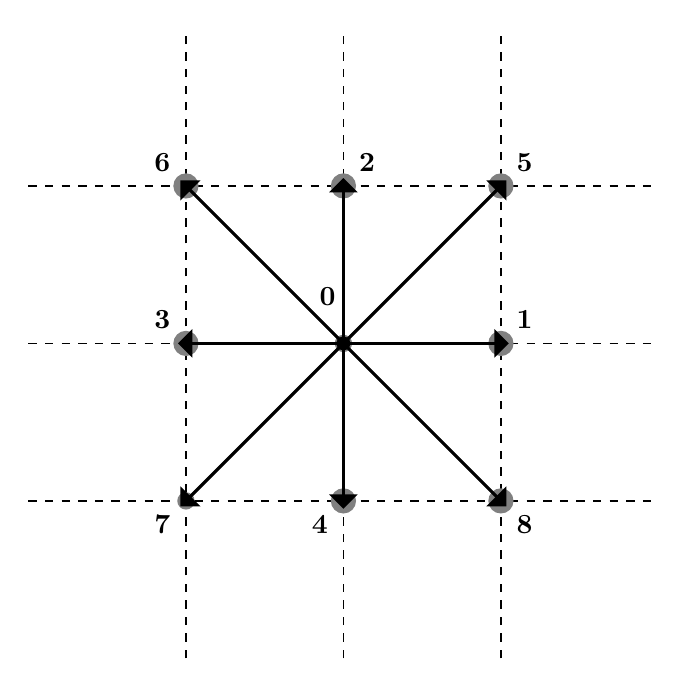
\begin{tikzpicture}[line width=0.2mm]

%\draw [dashed,line width=0.5mm] (0,0) rectangle(12,8);
\draw[dashed] (2,2) -- (10,2);
\draw[dashed] (2,4) -- (10,4);
\draw[dashed] (2,6) -- (10,6);
% \draw[dashed] (2,0) -- (2,8);
\draw[dashed] (4,0) -- (4,8);
\draw[dashed] (6,0) -- (6,8);
\draw[dashed] (8,0) -- (8,8);
% \draw[dashed] (10,0) -- (10,8);

\draw[gray,fill=black] (6,4)node[]{} circle(0.1cm);
% \draw[gray,fill=gray] (2,2)node[]{} circle(0.15cm);
\draw[gray,fill=gray] (4,2)node[]{} circle(0.1cm);
\draw[gray,fill=gray] (6,2)node[]{} circle(0.15cm);
\draw[gray,fill=gray] (8,2)node[]{} circle(0.15cm);
% \draw[gray,fill=gray] (10,2)node[]{} circle(0.15cm);

% \draw[gray,fill=gray] (2,4)node[]{} circle(0.15cm);
\draw[gray,fill=gray] (4,4)node[]{} circle(0.15cm);
%\draw[black,fill=black] (6,4)node[]{} circle(0.15cm);
\draw[gray,fill=gray] (8,4)node[]{} circle(0.15cm);
% \draw[gray,fill=gray] (10,4)node[]{} circle(0.15cm);

% \draw[gray,fill=gray] (2,6)node[]{} circle(0.15cm);
\draw[gray,fill=gray] (4,6)node[]{} circle(0.15cm);
\draw[gray,fill=gray] (6,6)node[]{} circle(0.15cm);
\draw[gray,fill=gray] (8,6)node[]{} circle(0.15cm);
% \draw[gray,fill=gray] (10,6)node[]{} circle(0.15cm);


\path[draw=black,solid,line width=0.4mm,fill=black,preaction={-triangle 90,thick,draw,shorten >=-1mm}](6,4) -- (8,4);
\path[draw=black,solid,line width=0.4mm,fill=black,preaction={-triangle 90,thick,draw,shorten >=-1mm}](6,4) -- (4,4);
\path[draw=black,solid,line width=0.4mm,fill=black,preaction={-triangle 90,thick,draw,shorten >=-1mm}](6,4) -- (6,6);
\path[draw=black,solid,line width=0.4mm,fill=black,preaction={-triangle 90,thick,draw,shorten >=-1mm}](6,4) -- (6,2);
\path[draw=black,solid,line width=0.4mm,fill=black,preaction={-triangle 90,thick,draw,shorten >=-1mm}](6,4) -- (8,6);
\path[draw=black,solid,line width=0.4mm,fill=black,preaction={-triangle 90,thick,draw,shorten >=-1mm}](6,4) -- (4,6);
\path[draw=black,solid,line width=0.4mm,fill=black,preaction={-triangle 90,thick,draw,shorten >=-1mm}](6,4) -- (4,2);
\path[draw=black,solid,line width=0.4mm,fill=black,preaction={-triangle 90,thick,draw,shorten >=-1mm}](6,4) -- (8,2);

% \draw[white,fill=white] (6,4)node[]{} circle(0.3cm);
% \draw (6,4) circle [radius=0.3] node {$\mathbf{0}$};
\draw (5.8,4.6)node[]{$\mathbf{0}$};
\draw (8.3,4.3)node[]{$\mathbf{1}$};
\draw (6.3,6.3)node[]{$\mathbf{2}$};
\draw (3.7,4.3)node[]{$\mathbf{3}$};
\draw (5.7,1.7)node[]{$\mathbf{4}$};
\draw (8.3,6.3)node[]{$\mathbf{5}$};
\draw (3.7,6.3)node[]{$\mathbf{6}$};
\draw (3.7,1.7)node[]{$\mathbf{7}$};
\draw (8.3,1.7)node[]{$\mathbf{8}$};

% \draw (7.5,4.3)node[]{$\mathbf{f_1}$};
% \draw (5.7,5.5)node[]{$\mathbf{f_2}$};
% \draw (4.5,3.7)node[]{$\mathbf{f_3}$};
% \draw (6.3,2.5)node[]{$\mathbf{f_4}$};
% \draw (7.1,5.5)node[]{$\mathbf{f_5}$};
% \draw (4.4,5.2)node[]{$\mathbf{f_6}$};
% \draw (4.8,2.3)node[]{$\mathbf{f_7}$};
% \draw (7.6,2.8)node[]{$\mathbf{f_8}$};
\end{tikzpicture}
\caption{Lattice directions and corresponding velocities for D2Q9 model}
\label{fig:D2Q9 lattice model}
\end{figure}

\begin{figure}[t] %Needs to be modified!!!!!!!!!!!!!!!!
\centering
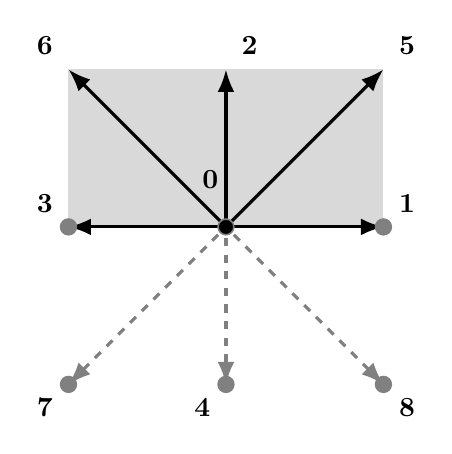
\begin{tikzpicture}[line width=0.2mm]


\fill[gray!30] (4,4) -- (8,4) -- (8,6) -- (4,6) -- cycle;




\draw[-Latex,shorten <=-2pt,solid,line width=0.4mm] (6,4) -- (8,4); %1
\draw[-Latex,shorten <=-2pt,solid,line width=0.4mm] (6,4) -- (4,4); %3
\draw[-Latex,shorten <=-2pt,solid,line width=0.4mm] (6,4) -- (6,6); %2
\draw[-Latex,shorten <=-2pt,dashed,gray,line width=0.4mm] (6,4) -- (6,2); %4
\draw[-Latex,shorten <=-2pt,solid,line width=0.4mm] (6,4) -- (8,6); %5
\draw[-Latex,shorten <=-2pt,solid,line width=0.4mm] (6,4) -- (4,6); %5
\draw[-Latex,shorten <=-2pt,dashed,gray,line width=0.4mm] (6,4) -- (4,2); %7
\draw[-Latex,shorten <=-2pt,dashed,gray,line width=0.4mm] (6,4) -- (8,2); %8



\draw (5.8,4.6)node[]{$\mathbf{0}$};
\draw (8.3,4.3)node[]{$\mathbf{1}$};
\draw (6.3,6.3)node[]{$\mathbf{2}$};
\draw (3.7,4.3)node[]{$\mathbf{3}$};
\draw (5.7,1.7)node[]{$\mathbf{4}$};
\draw (8.3,6.3)node[]{$\mathbf{5}$};
\draw (3.7,6.3)node[]{$\mathbf{6}$};
\draw (3.7,1.7)node[]{$\mathbf{7}$};
\draw (8.3,1.7)node[]{$\mathbf{8}$};

\draw[gray,fill=black] (6,4)node[]{} circle(0.1cm); %0
\draw[gray,fill=gray] (4,2)node[]{} circle(0.1cm);%7
\draw[gray,fill=gray] (6,2)node[]{} circle(0.1cm);%4
\draw[gray,fill=gray] (8,2)node[]{} circle(0.1cm);%8

\draw[gray,fill=gray] (4,4)node[]{} circle(0.1cm);%3
\draw[gray,fill=gray] (8,4)node[]{} circle(0.1cm);%1

% \draw[gray,fill=gray] (4,6)node[]{} circle(0.1cm);
% \draw[gray,fill=gray] (6,6)node[]{} circle(0.1cm);
% \draw[gray,fill=gray] (8,6)node[]{} circle(0.1cm);
% \draw[gray,fill=gray] (10,6)node[]{} circle(0.15cm);


% \draw (7.5,4.3)node[]{$\mathbf{f_1}$};
% \draw (5.7,5.5)node[]{$\mathbf{f_2}$};
% \draw (4.5,3.7)node[]{$\mathbf{f_3}$};
% \draw (6.3,2.5)node[]{$\mathbf{f_4}$};
% \draw (7.1,5.5)node[]{$\mathbf{f_5}$};
% \draw (4.4,5.2)node[]{$\mathbf{f_6}$};
% \draw (4.8,2.3)node[]{$\mathbf{f_7}$};
% \draw (7.6,2.8)node[]{$\mathbf{f_8}$};
\end{tikzpicture}
\caption{Edge}
\label{fig:D2Q9 lattice model}
\end{figure}

\begin{figure}[t] %Needs to be modified!!!!!!!!!!!!!!!!
\centering
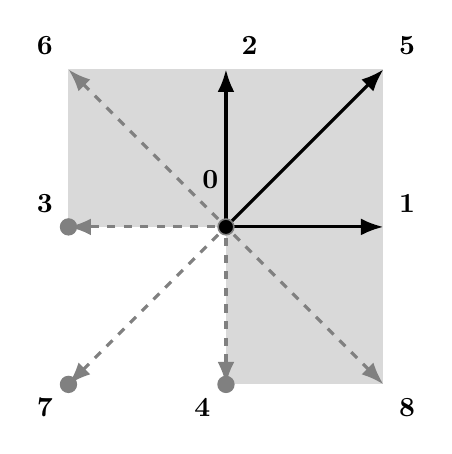
\begin{tikzpicture}[line width=0.2mm]


\fill[gray!30] (4,4) -- (8,4) -- (8,6) -- (4,6) -- cycle;
\fill[gray!30] (6,2) -- (8,2) -- (8,4) -- (6,4) -- cycle;




\draw[-Latex,shorten <=-2pt,solid,line width=0.4mm] (6,4) -- (8,4); %1
\draw[-Latex,shorten <=-2pt,dashed,gray,line width=0.4mm] (6,4) -- (4,4); %3
\draw[-Latex,shorten <=-2pt,solid,line width=0.4mm] (6,4) -- (6,6); %2
\draw[-Latex,shorten <=-2pt,dashed,gray,line width=0.4mm] (6,4) -- (6,2); %4
\draw[-Latex,shorten <=-2pt,solid,line width=0.4mm] (6,4) -- (8,6); %5
\draw[-Latex,shorten <=-2pt,dashed,gray,line width=0.4mm] (6,4) -- (4,6); %6
\draw[-Latex,shorten <=-2pt,dashed,gray,line width=0.4mm] (6,4) -- (4,2); %7
\draw[-Latex,shorten <=-2pt,dashed,gray,line width=0.4mm] (6,4) -- (8,2); %8



\draw (5.8,4.6)node[]{$\mathbf{0}$};
\draw (8.3,4.3)node[]{$\mathbf{1}$};
\draw (6.3,6.3)node[]{$\mathbf{2}$};
\draw (3.7,4.3)node[]{$\mathbf{3}$};
\draw (5.7,1.7)node[]{$\mathbf{4}$};
\draw (8.3,6.3)node[]{$\mathbf{5}$};
\draw (3.7,6.3)node[]{$\mathbf{6}$};
\draw (3.7,1.7)node[]{$\mathbf{7}$};
\draw (8.3,1.7)node[]{$\mathbf{8}$};

\draw[gray,fill=black] (6,4)node[]{} circle(0.1cm); %0
\draw[gray,fill=gray] (4,2)node[]{} circle(0.1cm);%7
\draw[gray,fill=gray] (6,2)node[]{} circle(0.1cm);%4
% \draw[gray,fill=gray] (8,2)node[]{} circle(0.1cm);%8

\draw[gray,fill=gray] (4,4)node[]{} circle(0.1cm);%3
% \draw[gray,fill=gray] (8,4)node[]{} circle(0.1cm);%1

% \draw[gray,fill=gray] (4,6)node[]{} circle(0.1cm);
% \draw[gray,fill=gray] (6,6)node[]{} circle(0.1cm);
% \draw[gray,fill=gray] (8,6)node[]{} circle(0.1cm);
% \draw[gray,fill=gray] (10,6)node[]{} circle(0.15cm);

\end{tikzpicture}
\caption{Corner}
\label{fig:D2Q9 lattice model}
\end{figure}




\end{document}



